\documentclass[11pt,oneside]{article}

\usepackage[T1]{fontenc}
\usepackage[utf8]{inputenc}
\usepackage{lmodern}
\usepackage{microtype}
\usepackage[a4paper,margin=1in]{geometry}
\usepackage{amsmath,amssymb,amsthm,mathtools}
\usepackage{bm}
\usepackage{booktabs,longtable,array,tabularx}
\usepackage{enumitem}
\usepackage{xcolor}
\usepackage{graphicx}
\usepackage{tikz}
\usetikzlibrary{arrows.meta,positioning,calc,shapes.geometric}
\usepackage{listings}
\usepackage{fancyhdr}
\usepackage{hyperref}
\usepackage[nameinlink,capitalise]{cleveref}

\definecolor{deepteal}{RGB}{0,91,96}
\definecolor{softteal}{RGB}{226,242,242}
\definecolor{deepblue}{RGB}{29,55,92}
\definecolor{softblue}{RGB}{232,239,249}
\definecolor{softgray}{RGB}{245,246,248}
\definecolor{brick}{RGB}{150,55,45}
\hypersetup{
  colorlinks=true,
  linkcolor=deepblue,
  citecolor=deepteal,
  urlcolor=brick,
  pdftitle={Alaoglu--Erdos Progress Report V: Synchronized-Gap Rigidity and Exact Local Lattice Costs},
  pdfauthor={OpenAI GPT-5.6 Pro}
}

\pagestyle{fancy}
\fancyhf{}
\fancyhead[L]{Alaoglu--Erd\H{o}s Progress Report V}
\fancyhead[R]{August 23, 2026}
\fancyfoot[C]{\thepage}
\setlength{\headheight}{14pt}

\setlength{\parindent}{0pt}
\setlength{\parskip}{0.58em}
\setlist[itemize]{leftmargin=1.65em,itemsep=0.25em,topsep=0.3em}
\setlist[enumerate]{leftmargin=1.8em,itemsep=0.25em,topsep=0.3em}
\renewcommand{\arraystretch}{1.15}

\newtheorem{theorem}{Theorem}[section]
\newtheorem{proposition}[theorem]{Proposition}
\newtheorem{lemma}[theorem]{Lemma}
\newtheorem{corollary}[theorem]{Corollary}
\newtheorem{conjecture}[theorem]{Conjecture}
\newtheorem{problem}[theorem]{Problem}
\newtheorem{criterion}[theorem]{Criterion}
\theoremstyle{definition}
\newtheorem{definition}[theorem]{Definition}
\newtheorem{remark}[theorem]{Remark}
\newtheorem{example}[theorem]{Example}

\newenvironment{resultbox}[1]{%
  \par\medskip\noindent
  \begin{minipage}{\linewidth}
  \hrule height 0.9pt\vspace{0.5em}
  {\color{deepteal}\bfseries #1}\par\smallskip
}{%
  \vspace{0.35em}\hrule height 0.9pt
  \end{minipage}\par\medskip
}

\newcommand{\Q}{\mathbb{Q}}
\newcommand{\Z}{\mathbb{Z}}
\newcommand{\R}{\mathbb{R}}
\newcommand{\C}{\mathbb{C}}
\newcommand{\F}{\mathbb{F}}
\newcommand{\Gm}{\mathbb{G}_{m}}
\newcommand{\vp}{v_p}
\newcommand{\ord}{\operatorname{ord}}
\newcommand{\height}{\operatorname{H}}
\newcommand{\hgt}{\operatorname{h}}
\newcommand{\lcm}{\operatorname{lcm}}
\newcommand{\supp}{\operatorname{supp}}
\newcommand{\rank}{\operatorname{rank}}
\newcommand{\diag}{\operatorname{diag}}
\newcommand{\covol}{\operatorname{covol}}
\newcommand{\im}{\operatorname{im}}
\newcommand{\kernel}{\operatorname{ker}}
\newcommand{\lgcd}{\operatorname{lgcd}}
\newcommand{\eps}{\varepsilon}
\newcommand{\ang}[1]{\left\langle #1\right\rangle}
\newcommand{\abs}[1]{\left|#1\right|}
\newcommand{\norm}[1]{\left\lVert#1\right\rVert}
\newcommand{\paren}[1]{\left(#1\right)}
\newcommand{\brak}[1]{\left[#1\right]}
\newcommand{\set}[1]{\left\{#1\right\}}

\lstdefinestyle{pythonstyle}{
  language=Python,
  basicstyle=\ttfamily\footnotesize,
  keywordstyle=\bfseries\color{deepblue},
  commentstyle=\itshape\color{deepteal},
  stringstyle=\color{brick},
  showstringspaces=false,
  frame=single,
  rulecolor=\color{black!25},
  backgroundcolor=\color{softgray},
  breaklines=true,
  columns=fullflexible,
  keepspaces=true,
  tabsize=4
}

\title{\vspace{-2.5em}
  {\LARGE\bfseries Synchronized-Gap Rigidity and Exact Local Lattice Costs}\\[0.45em]
  {\Large A Non-Duplicative Progress Report on the Alaoglu--Erd\H{o}s Conjecture}\\[0.9em]
  {\large Report V}}
\author{OpenAI GPT-5.6 Pro}
\date{August 23, 2026}

\begin{document}
\maketitle

\begin{abstract}
Assume hypothetically that a nonintegral real number $\beta$ satisfies
$M=2^\beta\in\Z$ and $A=3^\beta\in\Z$.  This report develops a new
frontier that is deliberately separate from the extensive reductions,
$p$-adic determinant experiments, interpolation arguments, Sturmian
codings, and auxiliary-function programs already present in the attached
unified report.  The principal global result proved here, conditional only
on a standard theorem of Levin on generalized greatest common divisors in
algebraic tori, is
\[
  \log\gcd\bigl(M^s-2^r,\,A^s-3^r\bigr)=o(r+s)
  \qquad (r+s\to\infty).
\]
Thus every synchronized pair of integer gaps has only a subexponential
common divisor.  An exceptional-subtorus descent is included; it is the
step needed to make the statement uniform on the whole rank-two orbit,
not merely away from an unspecified exceptional set.

The report then calculates the exact reduced height of the natural
synchronized quotient and proves that its approximation exponent to
$\log_2 3$ is asymptotically zero.  This closes a tempting rational-
approximation route.  On the local side, a Smith-normal-form calculation
gives the exact index of every $p$-adic exponent-congruence lattice.  At a
generic prime, $p^k$ of additional principal-unit precision costs
$p^{2k}$ exponent classes.  Minkowski's theorem converts this into a
precise ``square-root tax'': ordinary local lifting consumes two lattice
dimensions while the archimedean target has only one approximation
coordinate.  The resulting synthesis identifies the missing ingredient
as an adelic rank-transfer phenomenon, not simply stronger pointwise
lifting.  Several quantitatively stated targets, an exact Fermat-quotient
reconnaissance program, and a Lean formalization blueprint are supplied.
No complete proof of the conjecture is claimed.
\end{abstract}

\vspace{0.5em}
\begin{resultbox}{Status at a glance}
\begin{tabularx}{\linewidth}{@{}>{\bfseries}p{0.25\linewidth}X@{}}
New global theorem & Synchronized gaps have subexponential full gcd; the
prime-to-$6$ part follows from toric generalized-gcd theory and the primes
$2,3$ are controlled by $p$-adic logarithmic forms.\\
New exact calculation & The reduced quotient has height
$\exp\{s\log(M_0A_0)+o(s)\}$, so its convergence to $\log_2 3$ is far too
weak for irrationality-measure arguments.\\
New local accounting & Smith invariants give the exact congruence-lattice
index at every good prime and expose the generic quadratic cost.\\
Remaining bottleneck & A mechanism forcing coherent rank loss or a
macroscopic aggregate determinant defect across finite places.\\
Proof status & Substantial conditional progress, but not a proof of the
Alaoglu--Erd\H{o}s conjecture.\\
\end{tabularx}
\end{resultbox}

\tableofcontents
\newpage

\section{Scope, non-duplication, and public-status audit}

\subsection{What is and is not repeated}

The attached unified report is unusually comprehensive.  It already
contains the standard irrationality reduction, the conditional monoid of
integer values, primitive-valuation constructions, archimedean and
$p$-adic determinant programs, Fermat-quotient layers, Kummer-theoretic
reformulations, interpolation determinants, Subspace-Theorem barriers,
Sturmian encodings, and many quantified failure analyses.  Rephrasing
those chapters would add volume but not progress.

This report therefore uses only the common starting notation and develops
five pieces not presented there as a single rigorous mechanism:
\begin{enumerate}
  \item a global generalized-gcd theorem for the two synchronized gaps,
        including descent through every exceptional torus coset;
  \item an exact cancellation identity and height asymptotic for the
        natural quotient of those gaps;
  \item a Smith-normal-form law for the full tower of local exponent
        congruences, not merely its first determinant test;
  \item a geometry-of-numbers theorem translating local index into the
        best archimedean approximation one can force; and
  \item an adelic defect budget that states exactly how much exceptional
        local behavior would be needed to overcome the generic square law.
\end{enumerate}

The main purpose is diagnostic as well as constructive: each theorem
eliminates a vague hope and replaces it with a numerical target.

\subsection{Audit of the competitive claims}

The public record as of August 23, 2026 contains a manuscript by Elkies
and Klagsbrun constructing elliptic curves of rank at least $29$ and $30$,
with machine-checked components reported in the accompanying material
\cite{ElkiesKlagsbrun2026}.  It also contains a public 2026 manuscript and
seminar discussion proposing a counterexample to the Jacobian conjecture
\cite{Jacobian2026,Struppa2026}; a proposal of this scale should not be
confused with settled community consensus until the proof has survived
independent checking.  The ICARM Hadamard project publicly records the
completion of the formerly unresolved orders below $2000$ and provides
construction data \cite{ICARMHadamard2026}.

I found no public preprint, code repository, or formal proof announcing a
resolution of the Alaoglu--Erd\H{o}s conjecture.  The rival team's private
statement therefore cannot presently be audited.  The correct response is
not to infer a theorem from competitive pressure, but to make every new
claim below independently checkable.

\section{Conditional setup and synchronized gaps}\label{sec:setup}

Assume for the rest of the mathematical development that
\begin{equation}\label{eq:hyp-counterexample}
  \beta\in\R\setminus\Z,
  \qquad M:=2^\beta\in\Z_{>0},
  \qquad A:=3^\beta\in\Z_{>0}.
\end{equation}
A rational $\beta=u/v$ in lowest terms would make $2^{u/v}$ integral only
when $v=1$, so any counterexample is automatically irrational.  In
particular,
\begin{equation}\label{eq:real-log-relation}
  \frac{\log M}{\log 2}=\frac{\log A}{\log 3}=\beta,
  \qquad
  \log M\log 3-\log A\log 2=0.
\end{equation}
Neither $M$ is a power of $2$ nor $A$ a power of $3$.

For integers $r,s\ge1$ define the synchronized gaps
\begin{equation}\label{eq:gaps}
  D_2(r,s):=M^s-2^r,
  \qquad
  D_3(r,s):=A^s-3^r,
  \qquad
  \delta_{r,s}:=s\beta-r.
\end{equation}
They satisfy the exact archimedean identities
\begin{equation}\label{eq:gap-identities}
  D_2(r,s)=2^r\bigl(2^{\delta_{r,s}}-1\bigr),
  \qquad
  D_3(r,s)=3^r\bigl(3^{\delta_{r,s}}-1\bigr).
\end{equation}
When $r/s$ approximates $\beta$, the two gaps are simultaneously small
relative to their ambient powers.  Their common divisors are therefore a
natural place to look for a contradiction.

Two elementary facts will be used repeatedly.

\begin{lemma}[Multiplicative independence]\label{lem:independence}
Under \eqref{eq:hyp-counterexample}, the pairs $(2,3)$ and $(M,A)$ are
multiplicatively independent in the following strong sense: if
\[
  2^u3^v=1 \quad\text{or}\quad M^uA^v=1
  \qquad (u,v\in\Z),
\]
then $u=v=0$.
\end{lemma}

\begin{proof}
Unique factorization gives the assertion for $(2,3)$.  For $(M,A)$, take
real logarithms and use \eqref{eq:real-log-relation}:
$u\log M+v\log A=\beta(u\log2+v\log3)=0$.  As $\beta\ne0$, unique
factorization again gives $u=v=0$.
\end{proof}

\begin{lemma}[Polynomial lower bound for a synchronized error]
\label{lem:baker-delta}
There are effectively computable constants $C_0,C_1>0$, depending only on
$M$, such that whenever $r,s\ge1$ and $\delta_{r,s}\ne0$,
\begin{equation}\label{eq:baker-delta}
  \abs{\delta_{r,s}}
  \ge C_0\bigl(\max\{r,s\}\bigr)^{-C_1}.
\end{equation}
Consequently, along any sequence $r/s\to\beta$,
\begin{equation}\label{eq:small-gap-log}
  \log\abs{2^{\delta_{r,s}}-1}=o(s),
  \qquad
  \log\abs{3^{\delta_{r,s}}-1}=o(s).
\end{equation}
\end{lemma}

\begin{proof}
The nonzero linear form
$s\log M-r\log2=\delta_{r,s}\log2$ is a fixed-base linear form in two
logarithms.  A standard Baker--W\"ustholz estimate gives
$\abs{s\log M-r\log2}\gg\max\{r,s\}^{-C_1}$, proving
\eqref{eq:baker-delta}.  If $\delta=o(s)$, an elementary upper bound gives
$\log\abs{b^\delta-1\!}\le O(\abs\delta+1)=o(s)$ away from zero, while
\eqref{eq:baker-delta} gives the lower bound $-O(\log s)=o(s)$ near zero.
This proves \eqref{eq:small-gap-log} for $b=2,3$.
\end{proof}

\section{The rank-two torus orbit}\label{sec:torus-orbit}

Introduce the rational torus points
\begin{equation}\label{eq:orbit-point}
  P_{r,s}:=\bigl(M^s2^{-r},\,A^s3^{-r}\bigr)
  \in\Gm^2(\Q)
\end{equation}
and the finitely generated subgroup
\begin{equation}\label{eq:Gamma}
  \Gamma:=\ang{(2^{-1},3^{-1}),(M,A)}
  \subset\Gm^2(\Q).
\end{equation}
The map $(r,s)\mapsto P_{r,s}$ is injective: equality of two points would
give $2^{r-r'}=M^{s-s'}$, and irrationality of $\beta$ forces
$r=r'$ and $s=s'$.

\begin{proposition}[Zariski density]\label{prop:zariski-dense}
The subgroup $\Gamma$ is Zariski dense in $\Gm^2$.
\end{proposition}

\begin{proof}
The Zariski closure of a subgroup of a torus is an algebraic subgroup.  If
it were proper, some nontrivial character $X^uY^v$ would be trivial on its
identity component and, after taking a positive power, on $\Gamma$.  In
particular, evaluating on $(2^{-1},3^{-1})$ would give
$2^u3^v=1$.  By \cref{lem:independence}, $u=v=0$, a contradiction.
Equivalently, no nontrivial character vanishes identically on $\Gamma$.
\end{proof}

\subsection{Generalized gcd on a torus}

For rational numbers $x,y$, write the finite-place logarithmic gcd as
\begin{equation}\label{eq:finite-lgcd}
  \lgcd_{\mathrm{fin}}(x,y)
  :=\sum_{p}\min\bigl\{\max(0,\vp(x)),\max(0,\vp(y))\bigr\}\log p.
\end{equation}
For algebraic numbers one sums over normalized nonarchimedean places; a
full generalized gcd also includes archimedean proximity terms.  We need
only the consequence of Levin's theorem for the coprime Laurent
polynomials
\[
  f(X,Y)=X-1,
  \qquad g(X,Y)=Y-1.
\]
In the form used below, the theorem says that for every $\eps>0$, the
generalized gcd of $f(P)$ and $g(P)$ is at most $\eps\,h(P)$ for points
$P$ in a finitely generated subgroup, except on a finite union of
translates of proper subtori \cite{Levin2019,Xiao2022}.  Discarding
archimedean terms only weakens the estimate.

At a prime $p\ge5$, the denominators $2^r$ and $3^r$ in
\eqref{eq:orbit-point} are $p$-adic units.  Hence
\begin{align}
  \vp\bigl(M^s2^{-r}-1\bigr)&=\vp\bigl(D_2(r,s)\bigr),\label{eq:local-gap1}\\
  \vp\bigl(A^s3^{-r}-1\bigr)&=\vp\bigl(D_3(r,s)\bigr).
  \label{eq:local-gap2}
\end{align}
Thus the prime-to-$6$ common divisor of the integer gaps is exactly the
finite local gcd of the torus coordinates at the good primes.

\section{Global synchronized-gap rigidity}\label{sec:global-gcd}

A direct invocation of the toric theorem would leave an exceptional union
of torus cosets.  That is not enough: a hypothetical counterexample could
conceivably force every useful approximant into those cosets.  The next
argument descends through the exceptional set and is the main global
advance of this report.

\subsection{Pullback of exceptional cosets}

Let $C=\xi H$ be a translate of a proper subtorus $H\subset\Gm^2$.  If
$C\cap\Gamma$ is nonempty, choose $\gamma_0\in C\cap\Gamma$.  Then
\begin{equation}\label{eq:coset-intersection}
  C\cap\Gamma=\gamma_0(\Gamma\cap H).
\end{equation}
Because $\Gamma\cong\Z^2$ and is Zariski dense, $\Gamma\cap H$ has rank at
most one.  Under the injective exponent parametrization, the pullback of
$C\cap\Gamma$ is therefore either empty, a single point, or an affine
rank-one lattice
\begin{equation}\label{eq:affine-line}
  (r,s)=(r_0,s_0)+t(a,b),
  \qquad t\in\Z,
\end{equation}
for a nonzero primitive vector $(a,b)\in\Z^2$.

Along such a line,
\begin{equation}\label{eq:cyclic-line}
  P_{r,s}=(c_1\rho^t,c_2\sigma^t),
\end{equation}
where
\begin{equation}\label{eq:rho-sigma}
  c_1=M^{s_0}2^{-r_0},\quad c_2=A^{s_0}3^{-r_0},\quad
  \rho=M^b2^{-a},\quad \sigma=A^b3^{-a}.
\end{equation}

\begin{lemma}[Every exceptional line has a dense cyclic direction]
\label{lem:cyclic-dense}
For every nonzero $(a,b)\in\Z^2$, the numbers $\rho$ and $\sigma$ in
\eqref{eq:rho-sigma} are multiplicatively independent.  Hence
$\{(\rho^t,\sigma^t):t\in\Z\}$ is Zariski dense in $\Gm^2$.
\end{lemma}

\begin{proof}
Suppose $\rho^u\sigma^v=1$.  Taking real logarithms and using
\eqref{eq:real-log-relation} gives
\begin{align*}
  0
  &=u(b\log M-a\log2)+v(b\log A-a\log3)\\
  &=(b\beta-a)(u\log2+v\log3).
\end{align*}
Irrationality of $\beta$ and nonvanishing of $(a,b)$ imply
$b\beta-a\ne0$.  Therefore $2^u3^v=1$, so $u=v=0$.  A cyclic subgroup of
$\Gm^2$ is Zariski dense precisely when its two coordinates are
multiplicatively independent.
\end{proof}

\subsection{The prime-to-$6$ theorem}

For a nonzero integer $n$, let
\begin{equation}\label{eq:gcd6}
  n_{(6)}:=\frac{|n|}{2^{v_2(n)}3^{v_3(n)}},
  \qquad
  \gcd_{(6)}(u,v):=\gcd(u_{(6)},v_{(6)}).
\end{equation}

\begin{theorem}[Subexponential prime-to-$6$ synchronized gcd]
\label{thm:prime-to-six-gcd}
Under \eqref{eq:hyp-counterexample},
\begin{equation}\label{eq:prime-to-six-main}
  \log\gcd_{(6)}\bigl(D_2(r,s),D_3(r,s)\bigr)=o(r+s)
\end{equation}
as $r,s\ge1$ and $r+s\to\infty$.
Equivalently, for every $\eps>0$ there is $H_0(\eps,M,A)$ such that
\begin{equation}\label{eq:eps-gcd-bound}
  \gcd_{(6)}\bigl(D_2(r,s),D_3(r,s)\bigr)
  \le \exp\bigl(\eps(r+s)\bigr)
\end{equation}
whenever $r+s\ge H_0$.
\end{theorem}

\begin{proof}
Fix $\eps>0$.  Apply Levin's toric generalized-gcd theorem to the
Zariski-dense group $\Gamma$ and the coprime functions $X-1,Y-1$.  Outside
a finite union $Z_\eps$ of translates of proper subtori,
\begin{equation}\label{eq:levin-outside}
  \lgcd_{\mathrm{fin}}(P_1-1,P_2-1)
  \le \eps' h(P)
\end{equation}
for an $\eps'>0$ chosen below.  The logarithmic height of $P_{r,s}$ is
$O(r+s)$, with a constant depending only on $M,A$.  By
\eqref{eq:local-gap1}--\eqref{eq:local-gap2}, the contribution from
$p\ge5$ is exactly
$\log\gcd_{(6)}(D_2,D_3)$.  Choosing $\eps'$ small enough therefore gives
\eqref{eq:eps-gcd-bound} outside $Z_\eps$.

It remains to handle $P_{r,s}\in Z_\eps$.  By
\eqref{eq:coset-intersection}, the exponent pairs in this intersection
lie in finitely many points and affine lines of the form
\eqref{eq:affine-line}.  Isolated points are irrelevant asymptotically.
Fix one line.  The points have the cyclic form \eqref{eq:cyclic-line}, and
\cref{lem:cyclic-dense} says that its direction $(\rho,\sigma)$ is
Zariski dense.

Apply the same generalized-gcd theorem to the finitely generated subgroup
generated by $(c_1,c_2)$ and $(\rho,\sigma)$.  It gives a second finite
exceptional union of proper torus cosets.  Each such coset meets the
sequence $(c_1\rho^t,c_2\sigma^t)$ only finitely often: if it contained
two terms with parameters $t_1\ne t_2$, then
$(\rho,\sigma)^{t_1-t_2}$ would lie in a proper subtorus, contradicting
the Zariski density of its cyclic powers.  Thus, after finitely many
values of $t$, the generalized gcd on this line is $o(|t|)$.

There are only finitely many first-stage exceptional lines.  Taking the
maximum of their finite thresholds and rescaling $\eps'$ by the finitely
many height constants yields a uniform $o(r+s)$ estimate on all of them.
Combining the generic region, the exceptional lines, and the isolated
points proves the theorem.
\end{proof}

\begin{remark}[Why the second descent matters]
The conclusion is not a routine restatement of ``gcd is small outside an
exceptional set.''  The first exceptional set depends on $\eps$ and may
contain infinitely many exponent pairs.  The cyclic-density argument
shows that every rank-one component carries a fresh Zariski-dense orbit,
so the exceptional mechanism cannot persist after one descent.  In a
two-dimensional torus, the descent terminates.
\end{remark}

\subsection{Restoring the structural primes}

The denominator choices in \eqref{eq:orbit-point} single out $2$ and $3$.
They are not controlled by the preceding toric identity, but they are
much easier.

\begin{proposition}[Structural-prime contribution]\label{prop:structural-primes}
There is a constant $C=C(M,A)>0$ such that
\begin{equation}\label{eq:structural-bound}
  \min\{v_2(D_2),v_2(D_3)\}
  +\min\{v_3(D_2),v_3(D_3)\}
  \le C\bigl(1+\log(r+s)\bigr)^2.
\end{equation}
\end{proposition}

\begin{proof}
For the prime $2$, the common valuation is at most $v_2(A^s-3^r)$.  If
$A$ is even, this difference is odd and the valuation is zero.  If $A$ is
odd, then $A$ and $3$ are multiplicatively independent; otherwise
$A=3^m$ and \eqref{eq:real-log-relation} would give $\beta=m\in\Z$.
A fixed-base $2$-adic linear-form estimate therefore gives
$v_2(A^s-3^r)\ll(1+\log(r+s))^2$.

Similarly, the common $3$-adic valuation is at most $v_3(M^s-2^r)$.  It
is zero when $3\mid M$, and otherwise the multiplicative independence of
$M$ and $2$, followed by a fixed-base $3$-adic logarithmic-form estimate,
gives the same polylogarithmic bound.  Standard results of Yu or of
Bugeaud--Laurent are more than sufficient here \cite{Yu1998,BL1996}.
\end{proof}

\begin{theorem}[Full synchronized-gap rigidity]\label{thm:full-gcd}
Under \eqref{eq:hyp-counterexample},
\begin{equation}\label{eq:full-gcd-main}
  \boxed{\displaystyle
  \log\gcd\bigl(M^s-2^r,\,A^s-3^r\bigr)=o(r+s).}
\end{equation}
\end{theorem}

\begin{proof}
The prime-to-$6$ contribution is $o(r+s)$ by
\cref{thm:prime-to-six-gcd}; the two remaining local contributions are
$O((\log(r+s))^2)=o(r+s)$ by \cref{prop:structural-primes}.
\end{proof}

\begin{resultbox}{Interpretation of the global theorem}
No sequence of synchronized gaps can carry a common divisor of size
$\exp(c(r+s))$ for a fixed $c>0$.  Any proof strategy that tries to force
many local congruences simultaneously must therefore pay enough exponent
height to keep the total forced divisor subexponential.  The theorem does
not itself contradict the existence of $\beta$; it supplies a global
conservation law against which every local construction can be measured.
\end{resultbox}

\section{Exact cancellation and the height of the synchronized quotient}
\label{sec:height}

A natural reaction to \eqref{eq:gap-identities} is to divide the two small
gaps.  If $\delta_{r,s}\to0$, then
\begin{equation}\label{eq:natural-ratio}
  R_{r,s}
  :=\frac{A^s/3^r-1}{M^s/2^r-1}
  =\frac{3^{\delta_{r,s}}-1}{2^{\delta_{r,s}}-1}
  \longrightarrow \frac{\log3}{\log2}.
\end{equation}
Since $R_{r,s}\in\Q$, one might hope for rational approximations too good
for the known irrationality measure of $\log_2 3$.  The following exact
height calculation shows why that hope fails.

Write
\begin{equation}\label{eq:primitive-parts}
  a:=v_2(M),\qquad b:=v_3(A),\qquad
  M_0:=M/2^a,\qquad A_0:=A/3^b.
\end{equation}
Because $\beta$ is not an integer, $M_0>1$ and $A_0>1$.  Indeed,
$M_0=1$ would make $M=2^a$ and hence $\beta=a$; similarly for $A_0$.
Moreover
\begin{equation}\label{eq:beta-parts}
  \beta=a+\log_2 M_0=b+\log_3 A_0,
\end{equation}
so $\beta>a,b$.

For any sequence $s\to\infty$ with $r/s\to\beta$, eventually $r>as$ and
$r>bs$.  Define
\begin{equation}\label{eq:E2E3}
  E_2(r,s):=M_0^s-2^{r-as},
  \qquad
  E_3(r,s):=A_0^s-3^{r-bs}.
\end{equation}
Then $E_2$ is odd and $3\nmid E_3$, while
\begin{equation}\label{eq:Dfactor}
  D_2=2^{as}E_2,
  \qquad D_3=3^{bs}E_3.
\end{equation}

\begin{proposition}[Exact reduction identity]\label{prop:exact-reduction}
For $r>as,bs$, one has
\begin{equation}\label{eq:R-factor}
  R_{r,s}
  =\frac{2^{r-as}E_3(r,s)}{3^{r-bs}E_2(r,s)}.
\end{equation}
If $g_{r,s}:=\gcd_{(6)}(D_2,D_3)$, then the numerator and denominator on
the right of \eqref{eq:R-factor} have greatest common divisor exactly
$g_{r,s}$.  Consequently the reduced numerator and denominator are
\begin{equation}\label{eq:reduced-PQ}
  P_{r,s}=\frac{2^{r-as}|E_3|}{g_{r,s}},
  \qquad
  Q_{r,s}=\frac{3^{r-bs}|E_2|}{g_{r,s}}.
\end{equation}
\end{proposition}

\begin{proof}
Starting with \eqref{eq:natural-ratio},
\[
  R_{r,s}
  =\frac{2^r(A^s-3^r)}{3^r(M^s-2^r)}
  =\frac{2^{r-as}E_3}{3^{r-bs}E_2},
\]
which proves \eqref{eq:R-factor}.  Since $E_2$ is odd, the denominator has
no factor $2$ in common with the numerator.  Since $3\nmid E_3$, there is
no common factor $3$.  At every prime $p\ge5$, the common valuation is
$\min\{v_p(E_2),v_p(E_3)\}=\min\{v_p(D_2),v_p(D_3)\}$.  This is exactly
$g_{r,s}$.
\end{proof}

\begin{theorem}[Exact logarithmic height asymptotic]\label{thm:height-asymptotic}
Let $s\to\infty$ and $r/s\to\beta$.  In lowest terms, the rational number
$R_{r,s}$ has multiplicative height
\begin{equation}\label{eq:height-asymptotic}
  \boxed{\displaystyle
  \log\height(R_{r,s})
  =s\log(M_0A_0)+o(s).}
\end{equation}
More precisely,
\begin{equation}\label{eq:PQ-asymptotic}
  \log P_{r,s}=s\log(M_0A_0)+o(s),
  \qquad
  \log Q_{r,s}=s\log(M_0A_0)+o(s).
\end{equation}
\end{theorem}

\begin{proof}
Using $M_0^s=2^{s(\beta-a)}$ and $A_0^s=3^{s(\beta-b)}$,
\begin{align}
  E_2&=2^{r-as}\bigl(2^{\delta_{r,s}}-1\bigr),
  \label{eq:E2delta}\\
  E_3&=3^{r-bs}\bigl(3^{\delta_{r,s}}-1\bigr).
  \label{eq:E3delta}
\end{align}
By \cref{lem:baker-delta}, the logarithms of the final factors in
\eqref{eq:E2delta}--\eqref{eq:E3delta} are $o(s)$.  Since $r/s\to\beta$,
\begin{align}
  \log|E_2|
   &=(r-as)\log2+o(s)
    =s\log M_0+o(s),\label{eq:E2height}\\
  \log|E_3|
   &=(r-bs)\log3+o(s)
    =s\log A_0+o(s).\label{eq:E3height}
\end{align}
The global theorem \cref{thm:prime-to-six-gcd} gives
$\log g_{r,s}=o(r+s)=o(s)$.  Substitution into
\eqref{eq:reduced-PQ} yields
\begin{align*}
 \log P_{r,s}
 &= (r-as)\log2+\log|E_3|-\log g_{r,s}\\
 &=s\log M_0+s\log A_0+o(s),
\end{align*}
and the same calculation gives the formula for $Q_{r,s}$.
\end{proof}

\subsection{The rational-approximation route is quantitatively closed}

Set
\begin{equation}\label{eq:Fdelta}
  F(t):=\frac{3^t-1}{2^t-1},
  \qquad
  \theta:=\frac{\log3}{\log2}.
\end{equation}
The removable singularity of $F$ at $0$ has expansion
\begin{equation}\label{eq:Fexpansion}
  F(t)
  =\theta+\frac{\theta(\log3-\log2)}{2}\,t+O(t^2).
\end{equation}

\begin{corollary}[Zero power-of-height exponent]\label{cor:zero-exponent}
Along every sequence with $r/s\to\beta$ and $\delta_{r,s}\to0$,
\begin{equation}\label{eq:zero-exponent}
  \frac{-\log|R_{r,s}-\theta|}{\log\height(R_{r,s})}
  \longrightarrow0.
\end{equation}
In particular, for every fixed $\mu>0$ and all sufficiently large terms,
\begin{equation}\label{eq:no-height-power}
  |R_{r,s}-\theta|>\height(R_{r,s})^{-\mu}.
\end{equation}
\end{corollary}

\begin{proof}
The coefficient of $t$ in \eqref{eq:Fexpansion} is nonzero.  Therefore,
for sufficiently small nonzero $t$, $|F(t)-\theta|\asymp|t|$.  The Baker
lower bound \eqref{eq:baker-delta} implies
$-\log|\delta_{r,s}|=O(\log s)$.  On the other hand,
\cref{thm:height-asymptotic} gives
$\log\height(R_{r,s})=s\log(M_0A_0)+o(s)$, with a positive leading
constant.  Their ratio tends to zero.
\end{proof}

\begin{resultbox}{A closed door, not merely a failed estimate}
The quotient $R_{r,s}$ does converge to $\log_2 3$ whenever
$s\beta-r\to0$, but its numerator and denominator each retain essentially
all of the primitive exponential mass $M_0^sA_0^s$.  The common-gap gcd is
too small to cancel that mass.  Hence the approximation is logarithmic in
its height, not a positive power of its height.  Improvements to the
irrationality measure of $\log_2 3$ cannot rescue this particular route.
\end{resultbox}

\section{Exact local congruence lattices}\label{sec:smith}

The global theorem says that common divisibility cannot be too cheap in
aggregate.  We now calculate the local price exactly.  This section uses
only elementary $p$-adic Lie theory and Smith normal form.

Fix a prime
\begin{equation}\label{eq:good-prime}
  p\ge5,\qquad p\nmid6MA.
\end{equation}
For a $p$-adic unit $u$, write
\begin{equation}\label{eq:teich-split}
  u=\omega_p(u)\ang{u}_p,
  \qquad
  \omega_p(u)^{p-1}=1,
  \qquad
  \ang{u}_p\in1+p\Z_p.
\end{equation}
The Iwasawa logarithm kills the Teichm\"uller factor and satisfies
$\log_p u\in p\Z_p$.  Define the normalized logarithm matrix
\begin{equation}\label{eq:Bp}
  B_p:=\frac1p
  \begin{pmatrix}
    -\log_p2 & \log_p M\\
    -\log_p3 & \log_p A
  \end{pmatrix}
  \in M_2(\Z_p).
\end{equation}
For $z=(r,s)^{\mathsf T}$,
\begin{equation}\label{eq:Bpz}
  B_pz
  =\frac1p
  \begin{pmatrix}
     s\log_pM-r\log_p2\\
     s\log_pA-r\log_p3
  \end{pmatrix}.
\end{equation}

\begin{definition}[Principal-unit exponent lattice]
For $k\ge0$, set
\begin{equation}\label{eq:Lambda-p-k}
  \Lambda_p(k)
  :=\set{z\in\Z^2:B_pz\in p^k\Z_p^2}.
\end{equation}
Membership is equivalent to the two principal-unit congruences
\begin{equation}\label{eq:principal-congruences}
  \ang{M}_p^s\ang{2}_p^{-r}\equiv1\pmod{p^{k+1}},
  \qquad
  \ang{A}_p^s\ang{3}_p^{-r}\equiv1\pmod{p^{k+1}}.
\end{equation}
\end{definition}

\subsection{The Smith-index law}

Let $x_+:=\max(x,0)$.  If $B_p$ has rank two, there are
$U,V\in\mathrm{GL}_2(\Z_p)$ and uniquely determined integers
$0\le\alpha_p\le\gamma_p$ such that
\begin{equation}\label{eq:SNF}
  U B_p V=\diag(p^{\alpha_p},p^{\gamma_p}).
\end{equation}
Then
\begin{equation}\label{eq:tau-def}
  \tau_p:=v_p(\det B_p)=\alpha_p+\gamma_p.
\end{equation}
For rank one, write the Smith form as $\diag(p^{\alpha_p},0)$.

\begin{theorem}[Exact local index]\label{thm:smith-index}
For every $k\ge0$:
\begin{enumerate}
  \item if $\rank B_p=2$, then
  \begin{equation}\label{eq:rank2-index}
    [\Z^2:\Lambda_p(k)]
    =p^{(k-\alpha_p)_+ +(k-\gamma_p)_+};
  \end{equation}
  in particular, for $k\ge\gamma_p$,
  \begin{equation}\label{eq:stable-rank2-index}
    [\Z^2:\Lambda_p(k)]=p^{2k-\tau_p};
  \end{equation}
  \item if $\rank B_p=1$ with nonzero invariant $p^{\alpha_p}$, then
  \begin{equation}\label{eq:rank1-index}
    [\Z^2:\Lambda_p(k)]=p^{(k-\alpha_p)_+};
  \end{equation}
  \item if $B_p=0$, then $\Lambda_p(k)=\Z^2$.
\end{enumerate}
\end{theorem}

\begin{proof}
Complete $\Z^2$ at $p$.  Since the defining condition has finite
$p$-power index, its index in $\Z^2$ equals the index of
\[
  \set{z\in\Z_p^2:B_pz\in p^k\Z_p^2}
\]
in $\Z_p^2$.  Multiplication by $U$ and $V$ in
\eqref{eq:SNF} preserves Haar measure and index.  For a diagonal entry
$p^e$, the condition $p^ex\in p^k\Z_p$ imposes
$x\in p^{(k-e)_+}\Z_p$ and therefore contributes
$p^{(k-e)_+}$.  Multiplying the independent coordinate contributions
gives \eqref{eq:rank2-index} and \eqref{eq:rank1-index}.  A zero diagonal
entry imposes no condition.
\end{proof}

\begin{corollary}[Generic quadratic law]\label{cor:generic-quadratic}
If $\det B_p\in\Z_p^\times$, then $\alpha_p=\gamma_p=0$ and
\begin{equation}\label{eq:generic-index}
  [\Z^2:\Lambda_p(k)]=p^{2k}
  \qquad(k\ge0).
\end{equation}
Thus $p^k$ of additional principal-unit precision costs $p^{2k}$ exponent
classes.
\end{corollary}

\begin{remark}[Defect versus rank collapse]\label{rem:defect-rank}
A finite determinant valuation $\tau_p>0$ gives only a fixed credit
$p^{\tau_p}$ once $k\ge\gamma_p$; the slope in $k$ remains $2$.  A true
rank-one identity $\det B_p=0$ changes the slope from $2$ to $1$.  This is
why a first-layer vanishing congruence is not by itself the phenomenon a
proof needs.  One must distinguish
\[
  \det B_p\equiv0\pmod p,
  \qquad v_p(\det B_p)\gg1,
  \qquad \det B_p=0\text{ in }\Q_p.
\]
They have qualitatively different asymptotic effects.
\end{remark}

\subsection{First-layer Fermat quotient}

For $p\nmid u$, define
\begin{equation}\label{eq:fermat-q}
  q_p(u):=\frac{u^{p-1}-1}{p}\pmod p.
\end{equation}
The standard congruence
\begin{equation}\label{eq:log-fermat}
  \frac{\log_pu}{p}\equiv-q_p(u)\pmod p
\end{equation}
turns the determinant of \eqref{eq:Bp} into a completely elementary
first-layer test.

\begin{proposition}[Fermat-quotient shadow]\label{prop:fermat-shadow}
Define
\begin{equation}\label{eq:Delta-p}
  \Delta_p(M,A)
  :=q_p(M)q_p(3)-q_p(A)q_p(2)\in\F_p.
\end{equation}
Then
\begin{equation}\label{eq:det-modp}
  \det B_p\equiv\Delta_p(M,A)\pmod p.
\end{equation}
Consequently, $\Delta_p(M,A)\ne0$ implies the exact generic law
$[\Z^2:\Lambda_p(k)]=p^{2k}$ for all $k$.
\end{proposition}

\begin{proof}
Modulo $p$, the four entries of $B_p$ are respectively
$q_p(2),-q_p(M),q_p(3),-q_p(A)$.  Taking the determinant gives
$q_p(M)q_p(3)-q_p(A)q_p(2)$.
\end{proof}

\subsection{Restoring the Teichm\"uller layer}

Principal-unit conditions do not by themselves imply the original
integer congruences.  Define the residue or torsion lattice
\begin{equation}\label{eq:T-p}
  T_p:=\set{(r,s)\in\Z^2:
    M^s\equiv2^r\pmod p,\quad A^s\equiv3^r\pmod p}.
\end{equation}
Let
\begin{equation}\label{eq:t-p}
  t_p:=[\Z^2:T_p].
\end{equation}
The homomorphism
\[
  (r,s)\longmapsto(M^s2^{-r},A^s3^{-r})
  \quad\text{in }(\F_p^\times)^2
\]
has kernel $T_p$, so
\begin{equation}\label{eq:t-bound}
  t_p\mid(p-1)^2.
\end{equation}
In particular, $p\nmid t_p$.

\begin{theorem}[Full local congruence index]\label{thm:full-local-index}
The exponent pairs satisfying
\begin{equation}\label{eq:full-p-congruences}
  M^s\equiv2^r\pmod{p^{k+1}},
  \qquad
  A^s\equiv3^r\pmod{p^{k+1}}
\end{equation}
form the lattice
\begin{equation}\label{eq:Cpk}
  C_p(k)=T_p\cap\Lambda_p(k),
\end{equation}
and
\begin{equation}\label{eq:full-index-product}
  [\Z^2:C_p(k)]
  =t_p[\Z^2:\Lambda_p(k)].
\end{equation}
\end{theorem}

\begin{proof}
The Teichm\"uller decomposition \eqref{eq:teich-split} separates the
mod-$p$ condition from the principal-unit condition, proving
\eqref{eq:Cpk}.  The indices of $T_p$ and $\Lambda_p(k)$ are coprime: the
first divides $(p-1)^2$ and the second is a power of $p$.  For finite-index
subgroups of an abelian group with coprime indices, the index of the
intersection is the product.
\end{proof}

\subsection{Several primes and the defect budget}

For a finite set $S$ of good primes and depths $\bm{k}=(k_p)_{p\in S}$,
set
\begin{equation}\label{eq:Lambda-S}
  \Lambda_S(\bm{k}):=\bigcap_{p\in S}\Lambda_p(k_p),
  \qquad
  G_S(\bm{k}):=\prod_{p\in S}p^{k_p}.
\end{equation}
Because the individual indices are powers of distinct primes, the
Chinese remainder theorem gives exact multiplication.

\begin{theorem}[Exact finite-place product law]\label{thm:finite-product}
One has
\begin{equation}\label{eq:finite-product-index}
  [\Z^2:\Lambda_S(\bm{k})]
  =\prod_{p\in S}[\Z^2:\Lambda_p(k_p)].
\end{equation}
If every $B_p$ has rank two and $k_p\ge\gamma_p$, then
\begin{equation}\label{eq:defect-product}
  [\Z^2:\Lambda_S(\bm{k})]
  =\prod_{p\in S}p^{2k_p-\tau_p}
  =\frac{G_S(\bm{k})^2}{E_S},
\end{equation}
where the aggregate determinant credit is
\begin{equation}\label{eq:defect-budget}
  E_S:=\prod_{p\in S}p^{\tau_p}.
\end{equation}
\end{theorem}

\begin{proof}
For each $p$, the quotient $\Z^2/\Lambda_p(k_p)$ is a finite $p$-group.
The natural map from $\Z^2$ to their product is surjective by the Chinese
remainder theorem applied to a common modulus, and its kernel is the
intersection.  This proves \eqref{eq:finite-product-index}; the stable
Smith formula \eqref{eq:stable-rank2-index} gives
\eqref{eq:defect-product}.
\end{proof}

\begin{remark}[Torsion factors across several primes]
For the full lattices $C_p(k_p)$, each local index is still given exactly
by \eqref{eq:full-index-product}.  Across distinct primes, however, the
prime-to-$p$ torsion factors $t_p$ need not be pairwise coprime, so their
intersection index is not automatically the product of all $t_p$.  This
bounded first layer is arithmetically important for constructing actual
gap divisibility, but it does not change the asymptotic $p$-power slope
that drives the square-root barrier.
\end{remark}

\section{Covolume conservation and the square-root tax}
\label{sec:minkowski}

The Smith law is local.  To use it, one must find a point in the resulting
exponent lattice whose slope $r/s$ is close to $\beta$.  This is a
geometry-of-numbers problem with an exact answer.

\begin{theorem}[Constrained Dirichlet theorem]\label{thm:constrained-dirichlet}
Let $\Lambda\subset\Z^2$ be a lattice of finite index $I$, let
$\beta\in\R\setminus\Q$, and let $Q>1$, $\eta>0$.  There exists a nonzero
$(r,s)\in\Lambda$ such that, after changing both signs if necessary,
\begin{equation}\label{eq:constrained-dirichlet}
  0<s\le(1+\eta)IQ,
  \qquad
  |s\beta-r|\le Q^{-1}.
\end{equation}
\end{theorem}

\begin{proof}
Consider the determinant-one linear map
\begin{equation}\label{eq:Tbeta}
  T_\beta(r,s):=(s,s\beta-r).
\end{equation}
The lattice $L=T_\beta(\Lambda)$ has covolume $I$.  Let
\[
  K=[-X,X]\times[-Y,Y],
  \qquad
  X=(1+\eta)IQ,
  \qquad
  Y=Q^{-1}.
\]
Its area is $4XY=4(1+\eta)I>4\covol(L)$.  Minkowski's convex-body theorem
produces a nonzero point $T_\beta(r,s)\in L\cap K$.  If $s=0$, then
$|r|=|s\beta-r|\le Q^{-1}<1$, forcing $r=0$, contrary to nonzero-ness.
Thus $s\ne0$; replacing $(r,s)$ by $(-r,-s)$ gives $s>0$.
\end{proof}

\begin{corollary}[Height form]\label{cor:height-form}
For every $H>(1+\eta)I$, the lattice $\Lambda$ contains a nonzero
$(r,s)$ with $0<s\le H$ and
\begin{equation}\label{eq:error-index-height}
  |s\beta-r|
  \le\frac{(1+\eta)I}{H}.
\end{equation}
\end{corollary}

\begin{proof}
Use \cref{thm:constrained-dirichlet} with
$Q=H/((1+\eta)I)$, decreasing $H$ infinitesimally if necessary to retain
the strict Minkowski inequality.
\end{proof}

\subsection{Generic local precision costs a square}

Apply \cref{cor:height-form} to the principal-unit lattice
$\Lambda_S(\bm{k})$.  In the stable rank-two regime,
\eqref{eq:defect-product} gives
\begin{equation}\label{eq:I-G-E}
  I=\frac{G^2}{E},
  \qquad G:=G_S(\bm{k}),\quad E:=E_S.
\end{equation}
Consequently, at exponent height $H$ one can force both local logarithmic
conditions and guarantee only
\begin{equation}\label{eq:square-root-tax}
  |s\beta-r|
  \lesssim\frac{G^2}{EH}.
\end{equation}
If every selected prime is generic, $E=1$ and the right side is
$G^2/H$.

This is the square-root tax.  To prescribe one $p$-adic coordinate to
precision $p^k$ costs $p^k$ classes; prescribing two independent
coordinates costs $p^{2k}$.  Yet the archimedean approximation asks only
for the one linear form $s\beta-r$ to be small.  The second local
condition consumes a full lattice dimension without adding a second
archimedean degree of freedom.

\begin{figure}[ht]
\centering
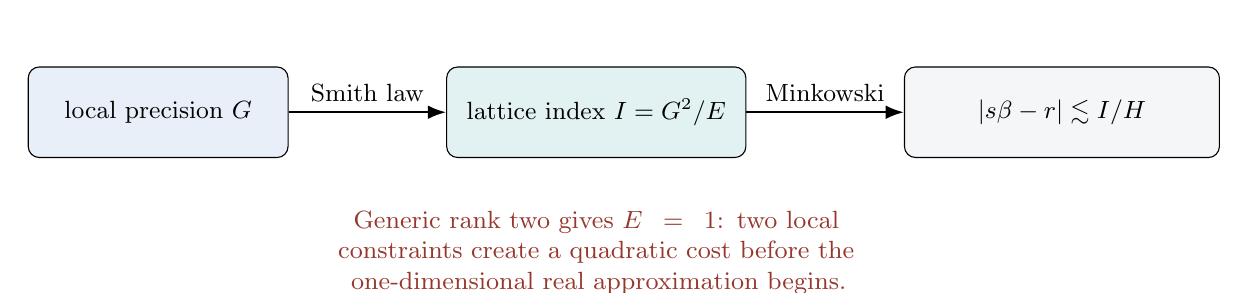
\begin{tikzpicture}[>=Latex, every node/.style={font=\small}]
  \node[draw,rounded corners,fill=softblue,minimum width=3.3cm,minimum height=1.15cm]
    (local) {local precision $G$};
  \node[draw,rounded corners,fill=softteal,minimum width=3.8cm,minimum height=1.15cm,
    right=2.0cm of local] (index) {lattice index $I=G^2/E$};
  \node[draw,rounded corners,fill=softgray,minimum width=4.0cm,minimum height=1.15cm,
    right=2.0cm of index] (arch) {$|s\beta-r|\lesssim I/H$};
  \draw[->,thick] (local) -- node[above]{Smith law} (index);
  \draw[->,thick] (index) -- node[above]{Minkowski} (arch);
  \node[below=0.55cm of index,text width=8.6cm,align=center,color=brick]
    {Generic rank two gives $E=1$: two local constraints create a quadratic
     cost before the one-dimensional real approximation begins.};
\end{tikzpicture}
\caption{The exact local-to-archimedean accounting chain.}
\label{fig:accounting-chain}
\end{figure}

\begin{proposition}[Defect needed to recover linear cost]
\label{prop:linear-cost}
In the full-rank stable regime, obtaining an essentially linear lattice
cost $I\le G^{1+o(1)}$ is equivalent to the aggregate condition
\begin{equation}\label{eq:linear-defect-condition}
  \log E\ge(1-o(1))\log G,
\end{equation}
or explicitly
\begin{equation}\label{eq:tau-budget-condition}
  \sum_{p\in S}\tau_p\log p
  \ge(1-o(1))\sum_{p\in S}k_p\log p.
\end{equation}
\end{proposition}

\begin{proof}
From \eqref{eq:I-G-E},
$\log I=2\log G-\log E$.  The assertion
$\log I\le(1+o(1))\log G$ is therefore exactly
\eqref{eq:linear-defect-condition}.
\end{proof}

\begin{remark}[Exact rank one]
If $B_p$ has rank one, then a depth $k$ costs only
$p^{k-\alpha_p}$ by \eqref{eq:rank1-index}.  At such a prime the quadratic
law genuinely collapses to a linear law.  A family of rank-one places would therefore be qualitatively different from a
family of isolated Fermat-quotient zeros with bounded $\tau_p$.  As
\cref{sec:compression} explains, even this slope change is not sufficient
without exceptional archimedean coherence of the surviving directions.
\end{remark}

\subsection{Why the volume calculation is the right benchmark}

The proof of \cref{thm:constrained-dirichlet} is elementary, but its
interpretive force is substantial.  The transformed lattice has
covolume $I$, while the target rectangle has side scales $H$ and
$|s\beta-r|$.  The area product must cross the covolume scale before
Minkowski can guarantee a nonzero point.  Thus any strategy that uses only
finite-index information and a symmetric convex-body argument will inherit
\begin{equation}\label{eq:area-conservation}
  H\cdot|s\beta-r|\asymp I.
\end{equation}
Escaping the square law therefore requires additional arithmetic structure
inside the lattice: unusually short directions, correlations among places,
or a genuine rank collapse.  A more elaborate convex body cannot create
such structure by itself.

\section{Global--local synthesis}\label{sec:synthesis}

The global theorem and the local index theorem describe the same tension
from opposite sides.

\subsection{Forced divisibility versus exponent height}

Suppose $(r,s)$ satisfies the full congruences
\begin{equation}\label{eq:forced-divisibility}
  M^s\equiv2^r\pmod N,
  \qquad
  A^s\equiv3^r\pmod N,
\end{equation}
where $N$ is supported on good primes.  Then
\begin{equation}\label{eq:N-gcd}
  N\mid\gcd(D_2(r,s),D_3(r,s)).
\end{equation}
The global theorem gives, along any sequence with $r+s\to\infty$,
\begin{equation}\label{eq:N-subexp}
  \log N=o(r+s).
\end{equation}
Thus an exponentially large forced modulus cannot occur at linearly
comparable exponent height.

On the other hand, the generic local law predicts that a principal-unit
modulus of scale $G$ has lattice index $G^2$.  Minkowski then naturally
finds exponents of size at least comparable to $G^2$ before obtaining a
fixed-quality real approximation.  At that height, $\log G$ is only
$O(\log(r+s))$, so \eqref{eq:N-subexp} is easily respected.  There is no
contradiction because the generic local construction is far more expensive
than the global theorem forbids.

\begin{resultbox}{The precise mismatch}
The global theorem rules out $N=\exp(cH)$ at exponent height $H$.
Generic local lifting produces only $N$ of polynomial size in $H$ because
the congruence lattice has index roughly $N^2$.  Between polynomial and
exponential lies a vast gap.  A proof needs a mechanism that changes the
local cost exponent, not a modest improvement in constants.
\end{resultbox}

\subsection{A phase diagram}

Let $G$ denote additional principal-unit precision, $E$ the determinant
credit, $I=G^2/E$ the exponent-lattice index, and $H$ the selected exponent
height.  The following regimes are qualitatively distinct.

\begin{longtable}{@{}p{0.21\linewidth}p{0.21\linewidth}p{0.24\linewidth}p{0.25\linewidth}@{}}
\toprule
Local regime & Index scale & Minkowski error at height $H$ & Assessment\\
\midrule
\endfirsthead
\toprule
Local regime & Index scale & Minkowski error at height $H$ & Assessment\\
\midrule
\endhead
Generic rank two & $I=G^2$ & $|\delta|\lesssim G^2/H$ & Too expensive; no tension with the global gcd theorem.\\
Finite defects & $I=G^2/E$, $E=G^{o(1)}$ & $|\delta|\lesssim G^{2-o(1)}/H$ & Same asymptotic slope; bounded-depth anomalies do not help.\\
Macroscopic defect & $E=G^{1-o(1)}$ & $|\delta|\lesssim G^{1+o(1)}/H$ & Removes one dimension of index cost; direction compression is still required.\\
Rank one at many places & $I\approx G$ & $|\delta|\lesssim G/H$ & A necessary structural shift, but insufficient without cross-prime short-direction coherence.\\
Rank zero & $I$ bounded & $|\delta|\lesssim H^{-1}$ & Would mean both $p$-adic logarithmic relations vanish identically; extraordinarily rigid.\\
\bottomrule
\end{longtable}

\subsection{The real determinant and its finite-place shadows}

The counterexample relation is the vanishing of the real determinant
\begin{equation}\label{eq:D-infty}
  D_\infty
  :=\det\begin{pmatrix}
    \log2&\log M\\
    \log3&\log A
  \end{pmatrix}
  =\log2\log A-\log3\log M=0.
\end{equation}
At a good finite prime define
\begin{equation}\label{eq:D-p}
  D_p
  :=\det\begin{pmatrix}
    \log_p2&\log_pM\\
    \log_p3&\log_pA
  \end{pmatrix}
  =-p^2\det B_p.
\end{equation}  The
conjecture asks, in effect, whether the real rank loss can occur without a
rational rank loss.  The local analysis shows that a proof would follow
from a sufficiently strong theorem transferring the archimedean rank loss
into aggregate finite-place rank loss.

There is no elementary product formula for the numbers $D_v$: each is a
bilinear expression in logarithms, not the valuation of a single algebraic
number.  This is exactly why the missing theorem is nontrivial.  Still,
\eqref{eq:D-infty} and \eqref{eq:D-p} organize the problem into an adelic
wedge:
\begin{equation}\label{eq:adelic-wedge}
  (\log_v2,\log_v3)\wedge(\log_vM,\log_vA),
  \qquad v\le\infty.
\end{equation}
The archimedean wedge vanishes.  A decisive principle would force that
vanishing to leave a quantitative trace among the finite wedges.

\section{New proof targets}\label{sec:targets}

This section turns the preceding accounting identities into explicit
research problems.  They are ordered by structural plausibility, not by
estimated difficulty.

\subsection{Target A: adelic defect transfer}

For arbitrary depth define the exact local Smith credit
\begin{equation}\label{eq:exact-depth-credit}
  e_p(k):=
  2k-\bigl((k-\alpha_p)_++(k-\gamma_p)_+\bigr)
  =\min(k,\alpha_p)+\min(k,\gamma_p).
\end{equation}
It is the exponent saved relative to the generic index $p^{2k}$.

\begin{conjecture}[Macroscopic defect transfer]\label{conj:defect-transfer}
Let integers $M,A>1$ satisfy $D_\infty=0$ but assume there is no rational
$q$ with $M=2^q$ and $A=3^q$.  Then there exist finite sets $S_j$ of good
primes and depths $k_{p,j}$ along which
\begin{equation}\label{eq:defect-transfer-target}
  \sum_{p\in S_j}e_p(k_{p,j})\log p
  \ge(1-o(1))\sum_{p\in S_j}k_{p,j}\log p.
\end{equation}
\end{conjecture}

The truncation in \eqref{eq:exact-depth-credit} is exact: Smith credit
beyond the requested depth cannot reduce the index further.  A version
strong enough to imply \eqref{eq:defect-transfer-target} would bring the
exponent-lattice index down to almost linear scale by
\cref{prop:linear-cost}; \cref{sec:compression} explains the additional
direction compression still required for a contradiction.

The conjecture is intentionally stated as a target, not asserted as a
known fact.  It resembles a four-logarithm or adelic linear-independence
principle, but its quantitative form is tailored to the exact amount of
credit required.  A weaker statement such as ``$\Delta_p=0$ for infinitely
many $p$'' is not enough: infinitely many isolated first-layer zeros can
still have zero density and bounded total credit.

\subsection{Target B: projective coherence of rank-one places}

Suppose $D_p=0$ and neither row of $B_p$ vanishes.  Then the two logarithm
vectors are proportional in $\Q_p^2$.  There is a projective slope
\begin{equation}\label{eq:cp}
  c_p
  =\frac{\log_pM}{\log_p2}
  =\frac{\log_pA}{\log_p3}
  \in\Q_p
\end{equation}
whenever the denominators are nonzero.  At the real place the analogous
slope is $\beta$.

A collection of rank-one primes is useful only if their one-dimensional
congruence directions are compatible in exponent space.  This motivates:

\begin{problem}[Moving-prime projective rigidity]\label{prob:projective-rigidity}
Show that if the slopes $c_p$ exist for a sufficiently rich set of primes
and the associated rank-one kernels admit exponent vectors of subquadratic
combined index, then the common real slope is rational, hence integral.
\end{problem}

One possible route is to construct rational approximants to the adelic
projective point $(c_v)_v$ and invoke a Subspace-Theorem statement on
$\mathbf P^1$ with moving local targets.  Unlike a direct application to
the gaps, this formulation retains the rank information that the Smith
law says is decisive.

\subsection{Target C: a second-order, not first-order, Fermat law}

The congruence $\Delta_p=0$ records only $v_p(D_p)\ge3$ in the unnormalized
determinant.  A proof needs information about the entire tower.  For
$u\in\Z_p^\times$ define higher logarithmic digits
\begin{equation}\label{eq:higher-digits}
  \lambda_{p,j}(u)
  :=p^{-j}\left(
      \log_pu-\sum_{i=1}^{j-1}p^i\lambda_{p,i}(u)
    \right)\pmod p.
\end{equation}
Equivalently, one may use Witt coordinates of the principal unit
$\ang{u}_p$.  Expanding $D_p$ digit by digit gives a hierarchy
\begin{equation}\label{eq:Witt-hierarchy}
  \Delta_p^{(1)},\Delta_p^{(2)},\ldots
\end{equation}
whose first term is \eqref{eq:Delta-p} and whose consecutive vanishing is
equivalent to increasing $\tau_p$.

\begin{problem}[Higher-layer correlation]
Derive a global relation among the sequences
$\lambda_{p,j}(2),\lambda_{p,j}(3),\lambda_{p,j}(M),\lambda_{p,j}(A)$ that
uses the real identity $D_\infty=0$ and forces either $D_p=0$ or a large
aggregate value of $\tau_p$ over a moving set of primes.
\end{problem}

This is a more accurate formulation than seeking many Wieferich-type
primes.  The objective is not first-digit vanishing but enough total
Smith credit to change the lattice-cost exponent.

\subsection{Target D: an auxiliary wedge with a product formula}

The obstacle to a direct adelic argument is that $D_v$ is not the
logarithm or valuation of one algebraic number.  A potentially overlooked
approach is to manufacture an algebraic auxiliary quantity whose first
nonzero local term is $D_v$.

For small formal parameters $X,Y$, consider the commutator-like expression
\begin{equation}\label{eq:aux-wedge}
  \Phi_v(X,Y)
  :=\bigl(2^X M^Y-1\bigr)\bigl(3^Y A^X-1\bigr)
   -\bigl(2^Y M^X-1\bigr)\bigl(3^X A^Y-1\bigr).
\end{equation}
Its lowest-order terms are alternating combinations of the two logarithm
vectors.  The raw expression in \eqref{eq:aux-wedge} is formal at present;
the research goal is to discretize $X,Y$ with integer interpolation or
finite differences so that:
\begin{enumerate}
  \item the resulting quantity is algebraic, preferably rational or
        integral;
  \item its archimedean size is unusually small because $D_\infty=0$;
  \item its $p$-adic valuation detects $\tau_p$; and
  \item the global product formula forces a nontrivial finite-place defect
        budget.
\end{enumerate}
This is not the usual interpolation determinant built from a single
exponential sequence.  The alternating construction is designed to
retain the two-by-two wedge that the local Smith analysis identifies.

\subsection{Target E: exploit the global gcd theorem contrapositive}

Theorem~\ref{thm:full-gcd} can be used as a contradiction engine if one
constructs synchronized exponents with a forced modulus $N$ satisfying
\begin{equation}\label{eq:contradiction-engine}
  \log N\ge c(r+s)
\end{equation}
for some fixed $c>0$.  Generic congruence lattices cannot do this, but a
rank-collapsed family might.  The exact target is therefore:

\begin{criterion}[A sufficient local construction]\label{crit:sufficient-local}
A contradiction follows if there exist exponent pairs $(r_j,s_j)$ and
good-prime moduli $N_j$ such that
\begin{equation}\label{eq:sufficient-local}
  N_j\mid D_2(r_j,s_j),\quad N_j\mid D_3(r_j,s_j),\quad
  \liminf_{j\to\infty}\frac{\log N_j}{r_j+s_j}>0.
\end{equation}
\end{criterion}

The criterion is immediate from \cref{thm:full-gcd}, but it focuses the
search: local progress matters only insofar as it approaches an
exponential divisor at linear exponent height.  Tables of isolated local
zeros should be evaluated against this threshold.

\section{Exact computational reconnaissance}\label{sec:computation}

A finite computation cannot test a nonexistent counterexample pair
$(M,A)$.  It can, however, audit the local formulas and calibrate how
special first-layer rank loss appears among nearby integer pairs.  The
following experiment scans the exact Fermat-quotient determinant
\eqref{eq:Delta-p}; it uses modular exponentiation modulo $p^2$, so no
floating-point arithmetic enters.

\subsection{Design of the scan}

The pair $(M,A)=(4,9)$ is an integral control corresponding to $\beta=2$.
For it, the real and every $p$-adic logarithm vector are exactly
proportional, hence $\Delta_p=0$ at every good prime.  The other pairs are
rough ``nearest-output'' proxies: $A$ was chosen loosely near the power-law curve suggested by the real relation, only to
sample arithmetic behavior, not because the pairs satisfy
$\log M/\log2=\log A/\log3$.  No statistical inference about a genuine
counterexample is made.

To avoid any ambiguity in that informal description, the computation is
best regarded simply as a fixed list of integer test pairs.  Its purposes
are:
\begin{itemize}
  \item verify the exact control identity;
  \item locate accidental first-layer zeros $\Delta_p=0$;
  \item illustrate that a zero at one prime is not the same as rank one in
        $\Q_p$; and
  \item provide reproducible input for future higher-layer scans.
\end{itemize}

\begin{table}[ht]
\centering
\small
\begin{tabular}{@{}rrrrlp{0.17\linewidth}@{}}
\toprule
$M$ & $A$ & good primes & first nonzero $\Delta_p$ & zero-defect primes below $1000$ & role\\
\midrule
4 & 9 & 166 & -- & all & integral control\\
5 & 13 & 164 & 7 & none & proxy\\
7 & 25 & 164 & 11 & 163 & proxy\\
11 & 41 & 164 & 5 & 7, 181 & proxy\\
13 & 55 & 163 & 7 & none & proxy\\
17 & 91 & 163 & 5 & none & proxy\\
19 & 119 & 163 & 5 & none & proxy\\
23 & 151 & 164 & 5 & 31, 251 & proxy\\
\bottomrule
\end{tabular}
\caption{Exact first-layer determinant scan.  ``Good'' means
$p\ge5$ and $p\nmid6MA$.  The integral control vanishes identically;
sporadic zeros for proxy pairs are only first-layer events.}
\label{tab:fermat-scan}
\end{table}

The control row is a useful implementation test: for $M=4$ and $A=9$,
$q_p(4)=2q_p(2)$ and $q_p(9)=2q_p(3)$ modulo $p$, so
$\Delta_p=0$ identically.  In the proxy rows, nonzero determinants appear
immediately or very early, while occasional isolated zeros occur.  The
proper conclusion is modest: generic full rank is common in unrelated
integer data, but first-layer accidents are not rare enough to carry
structural meaning by themselves.  A serious scan must compute
$\tau_p=v_p(\det B_p)$ or certify $D_p=0$ in $\Q_p$, rather than stop at
$\Delta_p$.

\subsection{Reproducibility}

The complete script is included in \cref{app:python}.  Its central line is
\[
  q_p(u)=\frac{u^{p-1}-1}{p}\pmod p,
\]
implemented by evaluating $u^{p-1}$ modulo $p^2$.  The table can therefore
be reproduced with standard Python alone.

\section{The second scale mismatch: index reduction is not yet compression}
\label{sec:compression}

The defect budget identifies when the local index drops from $G^2$ toward
$G$.  That is an important structural threshold, but it is not by itself
large enough to contradict the global gcd theorem.  The distinction is
best seen by writing
\begin{equation}\label{eq:L-logG}
  L:=\log G.
\end{equation}
Then the generic index is $e^{2L}$ and the rank-one index is $e^L$.
Minkowski's first theorem gives an unconstrained Euclidean short vector of
size at most a constant times $I^{1/2}$, hence of scale $e^L$ in the
generic case and $e^{L/2}$ in the rank-one case.  By contrast, a common
divisor of scale $G=e^L$ contradicts \cref{thm:full-gcd} only if the
associated exponent height is $O(L)$, or at least if $L/H$ stays bounded
away from zero.

Thus there are two separate compressions:
\begin{enumerate}
  \item \emph{dimension compression}: reduce the congruence index from
        $G^2$ toward $G$ by determinant defect or rank loss;
  \item \emph{direction compression}: produce a positive exponent vector
        of size $G^{o(1)}$, ideally $O(\log G)$, inside that lattice.
\end{enumerate}
The first is measured by Smith invariants.  The second is an archimedean
orientation problem across all selected finite places.  A successful
proof needs both, or a different mechanism that bypasses the congruence
lattice entirely.

\subsection{Positive minimum of a congruence lattice}

For a full-rank lattice $C\subset\Z^2$, define its positive minimum
\begin{equation}\label{eq:positive-minimum}
  \lambda_+(C):=
  \min\set{r+s:(r,s)\in C,\ r\ge1,\ s\ge1}.
\end{equation}
The minimum exists because a finite-index subgroup of $\Z^2$ contains a
positive multiple of each standard basis vector.

For a finite set of good primes with full depths $n_p\ge1$, let
\begin{equation}\label{eq:full-S-lattice}
  C_S(\bm n):=\bigcap_{p\in S}
  \set{(r,s):M^s\equiv2^r\pmod{p^{n_p}},\
                   A^s\equiv3^r\pmod{p^{n_p}}}
\end{equation}
and
\begin{equation}\label{eq:N-S}
  N_S(\bm n):=\prod_{p\in S}p^{n_p}.
\end{equation}

\begin{corollary}[No logarithmically short positive codeword]
\label{cor:no-short-codeword}
Under the hypothetical counterexample \eqref{eq:hyp-counterexample}, for
any sequence $(S_j,\bm n_j)$ with $N_j:=N_{S_j}(\bm n_j)\to\infty$,
\begin{equation}\label{eq:no-short-codeword}
  \frac{\log N_j}{\lambda_+(C_{S_j}(\bm n_j))}\longrightarrow0.
\end{equation}
\end{corollary}

\begin{proof}
Choose a positive minimizing vector $(r_j,s_j)$.  Then $N_j$ divides both
$D_2(r_j,s_j)$ and $D_3(r_j,s_j)$.  The heights $r_j+s_j$ must tend to
infinity: otherwise a bounded subsequence would contain a fixed positive
pair, while the nonzero fixed integer gcd of its two gaps could not be
divisible by $N_j\to\infty$.  Theorem~\ref{thm:full-gcd} now gives
\[
  \log N_j
  \le\log\gcd(D_2(r_j,s_j),D_3(r_j,s_j))
  =o(r_j+s_j),
\]
which is \eqref{eq:no-short-codeword}.
\end{proof}

This corollary recasts the global theorem as a minimum-distance law for a
family of arithmetic lattice codes.  Any local argument claiming a small
positive exponent vector can be checked against it immediately.

\subsection{Successive minima and the one-short-direction loophole}

Let $\lambda_1(C)\le\lambda_2(C)$ be Euclidean successive minima.  In
rank two, Minkowski's second theorem gives
\begin{equation}\label{eq:second-minkowski}
  \lambda_1(C)\lambda_2(C)\asymp [\Z^2:C]
\end{equation}
with absolute constants.  Therefore a lattice of very large index may
still contain one exceptionally short vector; the compensating second
vector is then very long.  Determinant calculations alone cannot exclude
this loophole.

For the Alaoglu--Erd\H{o}s problem, a single short vector shared by many
deep local congruences would already be striking.  If the same fixed
$(r,s)$ survived arbitrarily large depths at one prime, then
$M^s=2^r$ and $A^s=3^r$ as rational numbers, contradicting irrationality.
The more subtle possibility is a moving sequence of short directions.  A
new proof could attempt to show that the real rank relation
\eqref{eq:D-infty} prevents these directions from moving freely.

\begin{problem}[Cross-prime direction coherence]\label{prob:direction-coherence}
Prove an upper bound
\begin{equation}\label{eq:desired-compression}
  \lambda_+(C_S(\bm n))
  \le \bigl(\log N_S(\bm n)\bigr)^{O(1)}
\end{equation}
for an unbounded sequence of moduli forced by $D_\infty=0$, or prove a
weaker bound that still makes
$\log N_S/\lambda_+$ stay positive.  By
\cref{cor:no-short-codeword}, either conclusion rules out a
counterexample.
\end{problem}

The problem is deliberately strong.  It states the exact compression
needed, exposing why a mere density theorem for primes with
$\Delta_p=0$ would not finish the argument.

\subsection{Dual formulation}

Let $C^*:=\set{y\in\R^2:y\cdot C\subset\Z}$ be the Euclidean dual
lattice.  The linear form $s\beta-r$ corresponds to the vector
$(-1,\beta)$.  A small value on $C$ means that this real covector lies
close, in a suitable strip norm, to a rational covector from $C^*$.
Locally, the rows of $p^{-k}B_p$ generate the relevant modular dual
constraints.  Hence the missing adelic statement can also be phrased as:

\begin{problem}[Dual adelic approximation]
Use $D_\infty=0$ to show that the archimedean covector $(-1,\beta)$ is
unusually close to a dual vector assembled from the local logarithm rows,
with total denominator only polynomial in the requested depths rather
than exponential in their modulus.
\end{problem}

This dual viewpoint may be better suited to an adelic transference theorem
or to a geometry-of-numbers argument on an $S$-arithmetic lattice.  It
also suggests that the correct object is not a collection of unrelated
local kernels, but one global dual class whose local realizations are the
rows of $B_p$.

\section{Additional consequences of synchronized-gap rigidity}
\label{sec:consequences}

The global theorem has several useful corollaries beyond the quotient
height calculation.

\subsection{Weighted common valuation is negligible}

For every sequence $r+s\to\infty$,
\begin{equation}\label{eq:weighted-min-val}
  \sum_p\min\{v_p(D_2),v_p(D_3)\}\log p=o(r+s).
\end{equation}
Thus for any fixed $\eta>0$, the set of primes satisfying
\begin{equation}\label{eq:large-common-local}
  \min\{v_p(D_2),v_p(D_3)\}\log p\ge\eta(r+s)
\end{equation}
 is empty for all sufficiently large $(r,s)$.  More generally, no bounded
number of primes can carry a positive proportion of exponent height in
common valuation.

\subsection{Exponential coprime remainders}

Along $r/s\to\beta$, the individual gaps have logarithmic sizes
\begin{align}
  \log|D_2(r,s)|&=r\log2+o(s),\label{eq:D2-size}\\
  \log|D_3(r,s)|&=r\log3+o(s),\label{eq:D3-size}
\end{align}
provided $\delta_{r,s}=e^{-o(s)}$; this includes every sequence by
\cref{lem:baker-delta}.  Dividing by their gcd leaves
\begin{align}
  \log\frac{|D_2|}{\gcd(D_2,D_3)}&=r\log2+o(s),\\
  \log\frac{|D_3|}{\gcd(D_2,D_3)}&=r\log3+o(s).
\end{align}
Hence almost all exponential mass of each gap is carried by prime powers
not shared with the other gap.  Any prospective argument based on the
same prime support must therefore exploit unweighted support or residue
correlations, not a large common numerical factor.

\subsection{Fixed finite sets cannot dominate}

Fix a finite set of primes $S$.  Standard $p$-adic logarithmic-form
bounds give
\begin{equation}\label{eq:fixed-S}
  \sum_{p\in S}\min\{v_p(D_2),v_p(D_3)\}\log p
  =O_S((\log(r+s))^2).
\end{equation}
Thus every substantial common divisor must move to new primes.  This is a
precise moving-prime requirement: neither a single favorable prime nor a
fixed finite collection can generate the needed exponential scale.

\subsection{An entropy interpretation}

Let
\begin{equation}\label{eq:common-measure}
  \mu_{r,s}(p)
  :=\frac{\min\{v_p(D_2),v_p(D_3)\}\log p}{r+s}.
\end{equation}
Then \eqref{eq:weighted-min-val} says that the total mass
$\sum_p\mu_{r,s}(p)$ tends to zero.  Local lifting attempts to place mass
at selected primes, while the global theorem says the total common mass
vanishes.  The only possible escape is to use local data that does not
manifest as a common divisor---for example, correlated projective slopes,
local determinant defects, or auxiliary quantities with cancellation
before taking valuations.  This helps explain why the adelic wedge
\eqref{eq:adelic-wedge} is a more promising carrier of information than
the raw common factor alone.

\section{A formal proof-development plan in Lean}\label{sec:lean}

The new elementary and algebraic layers are well suited to formalization.
The deep toric generalized-gcd input is not currently a routine Mathlib
component, so a credible formal project should isolate it behind a clearly
named interface rather than silently axiomatize the final conjecture.

\subsection{Module graph}

\begin{center}
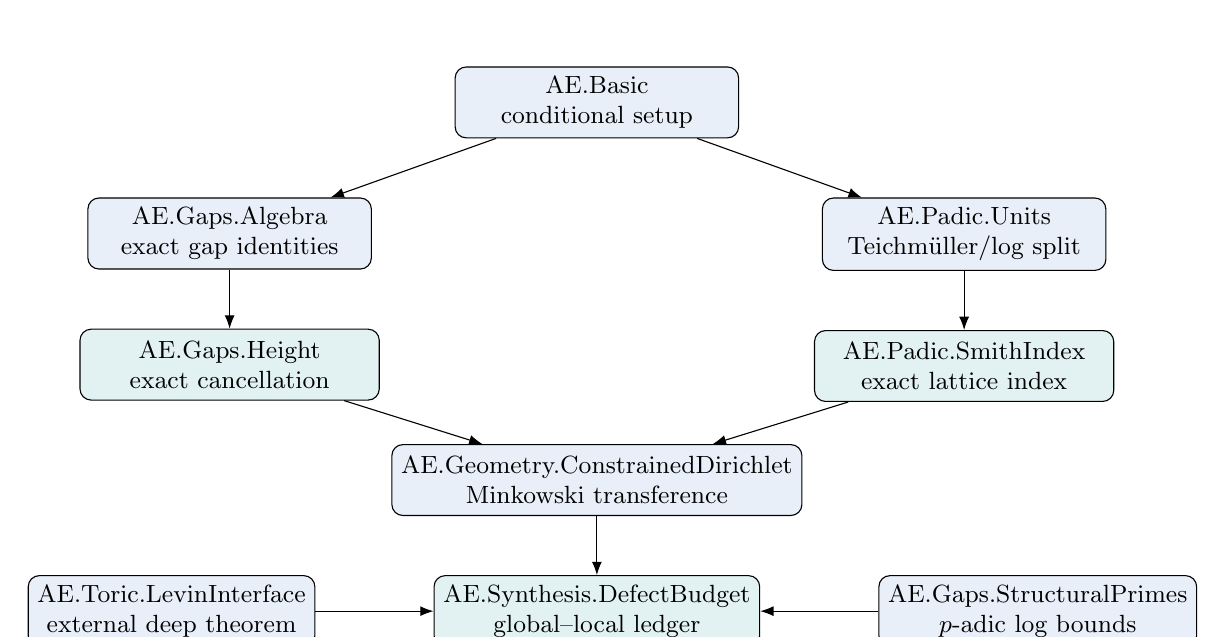
\begin{tikzpicture}[
  node distance=0.75cm and 1.05cm,
  box/.style={draw,rounded corners,fill=softblue,align=center,
              minimum width=3.6cm,minimum height=0.9cm,font=\small},
  deep/.style={draw,rounded corners,fill=softteal,align=center,
              minimum width=3.8cm,minimum height=0.9cm,font=\small},
  >=Latex]
\node[box] (basic) {AE.Basic\\conditional setup};
\node[box,below left=of basic] (gap) {AE.Gaps.Algebra\\exact gap identities};
\node[box,below right=of basic] (padic) {AE.Padic.Units\\Teichm\"uller/log split};
\node[deep,below=of gap] (height) {AE.Gaps.Height\\exact cancellation};
\node[deep,below=of padic] (smith) {AE.Padic.SmithIndex\\exact lattice index};
\node[box,below=1.0cm of $(height)!0.5!(smith)$] (mink) {AE.Geometry.ConstrainedDirichlet\\Minkowski transference};
\node[deep,below=of mink] (synth) {AE.Synthesis.DefectBudget\\global--local ledger};
\node[box,left=1.5cm of synth] (toric) {AE.Toric.LevinInterface\\external deep theorem};
\node[box,right=1.5cm of synth] (struct) {AE.Gaps.StructuralPrimes\\$p$-adic log bounds};
\draw[->] (basic)--(gap);
\draw[->] (basic)--(padic);
\draw[->] (gap)--(height);
\draw[->] (padic)--(smith);
\draw[->] (height)--(mink);
\draw[->] (smith)--(mink);
\draw[->] (mink)--(synth);
\draw[->] (toric)--(synth);
\draw[->] (struct)--(synth);
\end{tikzpicture}
\end{center}

\subsection{Core theorem signatures}

The following sketches use Mathlib-style names but are intentionally not
advertised as compiling code.  They specify the interfaces that a formal
implementation should realize.

\begin{lstlisting}[style=pythonstyle,language={},caption={Proposed Lean interfaces for the elementary core.}]
-- AE/Basic.lean
structure HypotheticalCounterexample where
  beta : Real
  M A : Nat
  hM : Real.rpow 2 beta = M
  hA : Real.rpow 3 beta = A
  hbeta : beta \notin Set.range ((Int.cast : Int -> Real))

-- AE/Padic/SmithIndex.lean
-- B is a 2 x 2 matrix over Z_p; smithExponents records alpha <= gamma.
theorem index_preimage_smith_rank_two
    (B : Matrix (Fin 2) (Fin 2) Zp)
    (hsmith : SmithData B alpha gamma)
    (k : Nat) :
    Fintype.card (ZModLatticeQuotient B k)
      = p ^ ((k - alpha) + (k - gamma)) := by
  ...

-- AE/Geometry/ConstrainedDirichlet.lean
theorem exists_lattice_approx
    (Lambda : Submodule Z (Fin 2 -> Z))
    (hfinite : FiniteIndex Lambda)
    (beta : Real) (hbeta : Irrational beta)
    (Q : Real) (hQ : 1 < Q) (eta : Real) (heta : 0 < eta) :
    exists r s : Z,
      vector![r,s] \in Lambda /\ 0 < s /\
      s <= (1+eta) * index Lambda * Q /\
      abs (s*beta-r) <= Q^(-1) := by
  ...

-- AE/Gaps/Height.lean
theorem reduced_gcd_eq_prime_to_six
    (h : HypotheticalCounterexample) (r s : Nat)
    (hr : valuation 2 h.M * s < r)
    (hs : valuation 3 h.A * s < r) :
    reducedCommonFactor (gap2 h r s) (gap3 h r s)
      = gcdPrimeToSix (gap2 h r s) (gap3 h r s) := by
  ...
\end{lstlisting}

The pseudo-code uses subtraction on natural numbers only schematically;
a real implementation should use truncated subtraction explicitly or
state the stable-depth theorem with hypotheses $k\ge\gamma$.

\subsection{Formalization order}

A sensible order minimizes dependence on difficult analysis:
\begin{enumerate}
  \item formalize the integer factorization identities
        \eqref{eq:Dfactor} and \eqref{eq:R-factor};
  \item formalize finite abelian-group indices and the coprime-intersection
        lemma used in \cref{thm:full-local-index};
  \item prove the Smith-index law first for diagonal matrices over
        $\Z/p^n\Z$, then transport through invertible row and column
        operations;
  \item formalize the determinant-one map $T_\beta$ and invoke the existing
        geometry-of-numbers infrastructure for Minkowski;
  \item isolate asymptotic facts about $o(s)$ and height in a separate
        file, with Baker's lower bound supplied as an imported theorem;
  \item represent Levin's theorem as a precisely scoped interface whose
        hypotheses include coprimality, finite generation, and the
        exceptional-subtorus conclusion;
  \item formalize the rank-one exceptional descent independently of the
        proof of Levin's theorem.
\end{enumerate}

The last item is especially valuable.  Even before the deep theorem is in
Mathlib, one can machine-check that its exceptional set is eliminated
correctly in this specific rank-two orbit.  That is the most delicate new
logical step in \cref{thm:prime-to-six-gcd}.

\subsection{What should not be hidden behind an axiom}

A formal artifact should not introduce an axiom equivalent to
``the synchronized gcd is subexponential.''  It should import only the
general toric gcd theorem and prove the following in Lean:
\begin{itemize}
  \item injectivity and Zariski density of the exponent orbit;
  \item rank at most one for intersections with proper subtori;
  \item multiplicative independence of every cyclic direction;
  \item finiteness of second-stage exceptional intersections;
  \item exact identification of good-prime local gcd terms; and
  \item reduction of the primes $2,3$ to fixed-base $p$-adic logarithmic
        forms.
\end{itemize}
This separation makes the formalization scientifically informative rather
than ceremonial.

\section{Limitations, verification boundaries, and next experiment}
\label{sec:limitations}

The report has intentionally separated theorem, conditional theorem,
conjectural target, and computation.  The boundaries are as follows.

\begin{enumerate}
  \item \textbf{No complete proof.}  The new results do not yet force
        $\beta\in\Z$.  They identify a sharper missing theorem.
  \item \textbf{Deep external input.}  The global gcd theorem uses Levin's
        generalized-gcd theorem on algebraic tori.  The exceptional-line
        descent is proved here, but the underlying toric theorem is not
        reproved.
  \item \textbf{Effectivity.}  The $o(r+s)$ estimate inherits the
        ineffectivity or poor effectivity of Subspace-Theorem technology.
        It supplies a structural asymptotic obstruction, not a practical
        numerical cutoff.
  \item \textbf{Structural primes.}  The primes $2$ and $3$ are controlled
        by standard $p$-adic logarithmic-form estimates.  Their precise
        constants are irrelevant to the asymptotic theorem and are not
        optimized.
  \item \textbf{Proxy computation.}  The pairs in
        \cref{tab:fermat-scan} do not satisfy the counterexample relation,
        except for the integral control.  The scan validates formulas and
        illustrates first-layer behavior; it is not statistical evidence
        for or against the conjecture.
  \item \textbf{Adelic targets.}  The defect-transfer and direction-
        coherence statements are proposed research targets.  They are not
        consequences of known four-logarithm theorems as presently stated.
\end{enumerate}

The most informative next computational experiment is not a wider scan of
$\Delta_p$.  It is a depth scan for the exact Smith data.  For each test
pair and prime, compute $B_p$ to precision $p^K$, determine
$\alpha_p,\gamma_p$, and compare the observed index of congruence solutions
modulo $p^k$ with \eqref{eq:rank2-index}.  The output should record
\begin{equation}\label{eq:next-experiment-output}
  (p,\alpha_p,\gamma_p,\tau_p,t_p,
   \lambda_+(C_p(k))_{1\le k\le K}).
\end{equation}
That experiment tests not only determinant depth but also the movement of
short exponent directions, the second compression identified in
\cref{sec:compression}.

\section{Conclusion}\label{sec:conclusion}

The central advance is a global rigidity law:
\[
  \log\gcd(M^s-2^r,A^s-3^r)=o(r+s).
\]
It says that synchronized gaps cannot share exponential mass.  The proof
uses the rank-two torus orbit, then explicitly descends through the finite
exceptional union by showing that every exceptional exponent line carries
a Zariski-dense cyclic direction.  This closes the usual exceptional-set
loophole.

The exact quotient-height theorem then shows that dividing the two gaps
does not create powerful rational approximations to $\log_2 3$: after all
cancellation, the height remains
$\exp\{s\log(M_0A_0)+o(s)\}$, while the error is only polynomially small
in $s$.

At finite places, the Smith law gives a complete local ledger.  Generic
additional precision $G$ costs index $G^2$; determinant defects contribute
an exact credit $E$; true rank loss changes the slope.  Minkowski's theorem
turns the index into an archimedean error and exposes the square-root tax.
A further comparison with the global gcd theorem reveals a second, more
severe mismatch: even an index of order $G$ does not automatically produce
positive exponent vectors of order $\log G$.  Cross-prime direction
coherence is therefore as important as rank loss.

The most promising unexplored route is an adelic wedge principle that
transfers the real determinant identity $D_\infty=0$ into both
macroscopic finite-place defect and coherent short directions.  The exact
thresholds are now stated in \eqref{eq:tau-budget-condition},
\eqref{eq:desired-compression}, and \cref{crit:sufficient-local}.  These
replace the open-ended instruction ``find more favorable primes'' with
quantitative success criteria.

\appendix

\section{Detailed exceptional-subtorus descent}\label{app:descent}

This appendix expands the uniformity argument in
\cref{thm:prime-to-six-gcd}, since that is the point most likely to be
underestimated in an informal proof.

\subsection{Characters and exponent kernels}

Every connected one-dimensional subtorus $H\subset\Gm^2$ is the kernel of
a primitive character
\begin{equation}\label{eq:character-H}
  \chi_{u,v}(X,Y)=X^uY^v,
  \qquad \gcd(u,v)=1.
\end{equation}
A translate $C=\xi H$ is cut out by
\begin{equation}\label{eq:translate-equation}
  X^uY^v=c
\end{equation}
for a nonzero algebraic constant $c$.  Pulling back along
$P_{r,s}$ gives
\begin{equation}\label{eq:pullback-character}
  2^{-ur}3^{-vr}M^{us}A^{vs}=c.
\end{equation}
If two exponent pairs $(r,s)$ and $(r',s')$ solve the same equation, their
difference $(R,S)=(r-r',s-s')$ satisfies
\begin{equation}\label{eq:kernel-character}
  2^{-uR}3^{-vR}M^{uS}A^{vS}=1.
\end{equation}
Thus the difference set is a subgroup of $\Z^2$.  It cannot have rank two,
for then $\Gamma$ would have a finite-index subgroup contained in $H$ and
its Zariski closure would be proper, contradicting
\cref{prop:zariski-dense}.  Hence it has rank at most one, proving the
affine-line description without invoking a general structure theorem for
intersections of finitely generated groups with cosets.

\subsection{A cyclic orbit meets a proper coset at most once after quotient}

Let $q=(\rho,\sigma)$ have multiplicatively independent coordinates and
consider $x_t=cq^t$.  If a proper torus coset $\xi H$ contains both
$x_{t_1}$ and $x_{t_2}$, then
\begin{equation}\label{eq:qdiff-H}
  q^{t_1-t_2}\in H.
\end{equation}
If $H$ is defined by $X^uY^v=1$, this gives
$(\rho^u\sigma^v)^{t_1-t_2}=1$.  Since $\rho,\sigma$ are positive rational
numbers in the present application, the only root of unity they can
produce is $1$, so $\rho^u\sigma^v=1$.  Multiplicative independence forces
$u=v=0$, contradicting properness of $H$.  Thus each proper coset contains
at most one term of the cyclic orbit.  For a finite union, the intersection
is finite with an explicit cardinality bounded by the number of cosets.

\subsection{Uniform little-$o$ across finitely many lines}

Fix a target $\eps>0$.  On the generic part of the rank-two group, apply
Levin with parameter $\eps/(3C_0)$, where
\begin{equation}\label{eq:height-C0}
  h(P_{r,s})\le C_0(r+s)+C_0.
\end{equation}
This gives the desired estimate outside finitely many cosets for large
$r+s$.

For each exceptional line $L_i$, write $(r,s)=(r_i,s_i)+t(a_i,b_i)$.
There are constants $c_i,C_i>0$ such that, outside finitely many $t$,
\begin{equation}\label{eq:t-height-equivalence}
  c_i|t|-C_i\le r+s\le C_i|t|+C_i
\end{equation}
when restricted to the positive quadrant.  Apply Levin to the cyclic
group on $L_i$ with parameter $\eps c_i/(3C_i')$, where $C_i'$ is a height
constant for $(c_1\rho^t,c_2\sigma^t)$.  After excluding the finite second-
stage intersections, the local gcd is at most $\eps(r+s)/3$ for all large
positive-quadrant points on $L_i$.

The number of lines is finite.  Taking the maximum of their thresholds,
and absorbing all isolated and initially excluded points into one finite
set, proves a single $H_0(\eps)$ valid on the entire orbit.  This is the
quantifier needed for \eqref{eq:prime-to-six-main}.

\section{Smith normal form and index details}\label{app:smith}

\subsection{One-dimensional calculation}

Let $e,k\ge0$.  The subgroup
\begin{equation}\label{eq:one-dim-preimage}
  L_{e,k}:=\set{x\in\Z_p:p^ex\in p^k\Z_p}
\end{equation}
is
\begin{equation}\label{eq:one-dim-result}
  L_{e,k}=p^{(k-e)_+}\Z_p,
  \qquad
  [\Z_p:L_{e,k}]=p^{(k-e)_+}.
\end{equation}
The two-dimensional formula is simply the product of two copies of
\eqref{eq:one-dim-result} after Smith reduction.

\subsection{Why integral and $p$-adic indices agree}

Let
\begin{equation}\label{eq:Z-lattice-condition}
  \Lambda=\set{z\in\Z^2:Bz\in p^k\Z_p^2}.
\end{equation}
The condition depends only on $z$ modulo a sufficiently high power $p^N$,
for example $N=k+\max(0,-\min v_p(B_{ij}))$ before normalization.  Hence
$\Lambda$ is the inverse image of a subgroup of $(\Z/p^N\Z)^2$.  Its
index equals the cardinality of the corresponding quotient.  Completing
at $p$ produces the same finite quotient because $\Z^2$ is dense in
$\Z_p^2$ and reduction modulo $p^N$ is surjective.  Thus no subtlety is
hidden in passing from $\Z^2$ to $\Z_p^2$ in
\cref{thm:smith-index}.

\subsection{Smith invariants from minors}

For a rank-two matrix $B\in M_2(\Z_p)$,
\begin{equation}\label{eq:smith-minors}
  \alpha=\min_{i,j}v_p(B_{ij}),
  \qquad
  \alpha+\gamma=v_p(\det B).
\end{equation}
Therefore a computation of $\tau=v_p(\det B)$ alone does not determine the
onset depth $\gamma$ unless the minimum entry valuation $\alpha$ is also
known.  In the common generic situation where at least one normalized
logarithm is a $p$-adic unit, $\alpha=0$ and $\gamma=\tau$.  Then
\begin{equation}\label{eq:index-alpha0}
  [\Z^2:\Lambda_p(k)]
  =p^{k+(k-\tau)_+}.
\end{equation}
The index initially grows with slope one until depth $\tau$, then with
slope two.  This finite initial interval is precisely what a
first-layer Fermat zero detects; it should not be mistaken for permanent
rank one.

\subsection{Torsion-principal separation}

The map
\begin{equation}\label{eq:residue-map}
  \varphi_p:\Z^2\to(\F_p^\times)^2,
  \qquad
  (r,s)\mapsto(M^s2^{-r},A^s3^{-r})
\end{equation}
has image of cardinality $t_p$ and kernel $T_p$.  The principal-unit map
at depth $k$ has a $p$-group image.  Since one image has order prime to
$p$ and the other has $p$-power order, the combined map has image the
direct product of the two images.  This gives a second proof of
\eqref{eq:full-index-product} and is a convenient formulation for Lean.

\section{Height calculation details}\label{app:height}

\subsection{Uniform control of $b^\delta-1$}

Let $\delta=o(s)$ be nonzero and satisfy $|\delta|\ge s^{-C}$.  For fixed
$b>1$:
\begin{itemize}
  \item if $|\delta|\le1$, the mean-value theorem gives
        $|b^\delta-1|\asymp_b|\delta|$, so its logarithm lies between
        $-C\log s+O(1)$ and $O(1)$;
  \item if $\delta>1$, then
        $0<\log(b^\delta-1)\le\delta\log b=o(s)$;
  \item if $\delta<-1$, then $|b^\delta-1|$ is bounded above and below by
        positive constants.
\end{itemize}
Hence $\log|b^\delta-1|=o(s)$ uniformly in all three regimes.  This is the
only analytic input needed after Baker's lower bound.

\subsection{Exact cancellation prime by prime}

For $p\ge5$,
\begin{align*}
 v_p\bigl(2^{r-as}E_3\bigr)&=v_p(E_3)=v_p(D_3),\\
 v_p\bigl(3^{r-bs}E_2\bigr)&=v_p(E_2)=v_p(D_2).
\end{align*}
At $p=2$, the denominator is odd; at $p=3$, the numerator is prime to $3$.
Therefore the reduced common factor is exactly
\[
  \prod_{p\ge5}p^{\min(v_p(D_2),v_p(D_3))},
\]
with no hidden cancellation at the structural primes.  This exactness is
what allows the global gcd theorem to feed directly into the height
asymptotic.

\section{Reproducible Fermat-quotient scan}\label{app:python}

\begin{lstlisting}[style=pythonstyle,caption={Exact script used for
\cref{tab:fermat-scan}.}]
#!/usr/bin/env python3
"""Exact first-layer p-adic determinant reconnaissance."""
from __future__ import annotations
from math import gcd


def primes_below(n: int) -> list[int]:
    sieve = bytearray(b"\x01") * n
    sieve[:2] = b"\x00\x00"
    for p in range(2, int(n**0.5) + 1):
        if sieve[p]:
            sieve[p*p:n:p] = b"\x00" * (((n-1-p*p)//p)+1)
    return [i for i in range(2, n) if sieve[i]]


def fermat_quotient(u: int, p: int) -> int:
    # Reducing modulo p^2 keeps the quotient exact.
    return ((pow(u, p - 1, p * p) - 1) // p) % p


def defect(M: int, A: int, p: int) -> int:
    qM = fermat_quotient(M, p)
    qA = fermat_quotient(A, p)
    q2 = fermat_quotient(2, p)
    q3 = fermat_quotient(3, p)
    return (qM * q3 - qA * q2) % p


def summarize(M: int, A: int, bound: int = 1000):
    good = [p for p in primes_below(bound)
            if p >= 5 and gcd(p, 6*M*A) == 1]
    zeros = [p for p in good if defect(M, A, p) == 0]
    first_nonzero = next(
        (p for p in good if defect(M, A, p) != 0), None)
    return len(good), zeros, first_nonzero


def main() -> None:
    pairs = [
        (4, 9, "integral control, beta=2"),
        (5, 13, "proxy"),
        (7, 25, "proxy"),
        (11, 41, "proxy"),
        (13, 55, "proxy"),
        (17, 91, "proxy"),
        (19, 119, "proxy"),
        (23, 151, "proxy"),
    ]
    for M, A, description in pairs:
        total, zeros, first = summarize(M, A)
        print(M, A, description, total, zeros, first)


if __name__ == "__main__":
    main()
\end{lstlisting}

\section{Checklist for independent verification}\label{app:checklist}

An independent reader can audit the new chain in the following order.

\begin{enumerate}
  \item Verify irrationality of a nonintegral hypothetical $\beta$ and the
        Zariski density of $\Gamma$.
  \item Check the statement of Levin's theorem for $X-1,Y-1$ on a finitely
        generated subgroup of $\Gm^2$.
  \item Verify that each first-stage exceptional coset pulls back to rank
        at most one in exponent space.
  \item Check the calculation
        $(b\beta-a)(u\log2+v\log3)=0$ on every exceptional line.
  \item Apply the toric theorem a second time and verify finite intersection
        with the new exceptional cosets.
  \item Check the $p=2,3$ reductions and invoke any standard fixed-base
        $p$-adic logarithmic-form bound.
  \item Verify the exact quotient factorization and cancellation at
        $2,3$.
  \item Check the Smith diagonal preimage one coordinate at a time.
  \item Verify the coprimality of torsion and principal indices.
  \item Apply Minkowski to the rectangle with area
        $4(1+\eta)I$.
\end{enumerate}

Every step except items 2 and 6 is elementary or algebraic.  Items 2 and 6
are standard external theorems with explicit references below.

\begin{thebibliography}{99}

\bibitem{AlaogluErdos1944}
L.~Alaoglu and P.~Erd\H{o}s,
\newblock On highly composite and similar numbers,
\newblock \emph{Transactions of the American Mathematical Society}
\textbf{56} (1944), 448--469.

\bibitem{BakerWustholz1993}
A.~Baker and G.~W\"ustholz,
\newblock Logarithmic forms and group varieties,
\newblock \emph{Journal f\"ur die reine und angewandte Mathematik}
\textbf{442} (1993), 19--62.

\bibitem{BL1996}
Y.~Bugeaud and M.~Laurent,
\newblock Minoration effective de la distance $p$-adique entre puissances
de nombres alg\'ebriques,
\newblock \emph{Journal of Number Theory} \textbf{61} (1996), 311--342.

\bibitem{BombieriGubler2006}
E.~Bombieri and W.~Gubler,
\newblock \emph{Heights in Diophantine Geometry},
\newblock Cambridge University Press, 2006.

\bibitem{BCZ2003}
Y.~Bugeaud, P.~Corvaja, and U.~Zannier,
\newblock An upper bound for the G.C.D. of $a^n-1$ and $b^n-1$,
\newblock \emph{Mathematische Zeitschrift} \textbf{243} (2003), 79--84.

\bibitem{ESS2002}
J.-H.~Evertse, H.~P.~Schlickewei, and W.~M.~Schmidt,
\newblock Linear equations in variables which lie in a multiplicative group,
\newblock \emph{Annals of Mathematics} \textbf{155} (2002), 807--836.

\bibitem{Levin2019}
A.~Levin,
\newblock Greatest common divisors and Vojta's conjecture for blowups of
algebraic tori,
\newblock \emph{Inventiones Mathematicae} \textbf{215} (2019), 493--533,
\newblock \href{https://doi.org/10.1007/s00222-018-0831-z}{doi:10.1007/s00222-018-0831-z}.

\bibitem{Xiao2022}
H.~Xiao,
\newblock Greatest common divisors and almost units on split algebraic tori,
\newblock \emph{Acta Arithmetica} \textbf{206} (2022), 195--222;
\newblock \href{https://arxiv.org/abs/2110.01751}{arXiv:2110.01751}.

\bibitem{Yu1998}
K.~Yu,
\newblock $p$-adic logarithmic forms and group varieties. III,
\newblock \emph{Forum Mathematicum} \textbf{10} (1998), 325--381.

\bibitem{ElkiesKlagsbrun2026}
N.~D.~Elkies and Z.~Klagsbrun,
\newblock Elliptic curves of rank 29 and 30,
\newblock preprint (2026),
\newblock \href{https://arxiv.org/abs/2603.04842}{arXiv:2603.04842}.

\bibitem{Jacobian2026}
Authors of arXiv:2602.20474,
\newblock A proposed counterexample concerning Keller's Jacobian conjecture,
\newblock preprint (2026),
\newblock \href{https://arxiv.org/abs/2602.20474}{arXiv:2602.20474}.

\bibitem{Struppa2026}
D.~C.~Struppa,
\newblock A counterexample to Keller's Jacobian Conjecture,
\newblock public seminar announcement, Chapman University, March 2, 2026.

\bibitem{ICARMHadamard2026}
Institute for Computational and Experimental Research in Mathematics
(ICARM),
\newblock Hadamard matrix orders and construction archive,
\newblock public project page, accessed August 23, 2026.

\end{thebibliography}

\end{document}
